\section{Circuito n° 3: Rectificador de precisión }

\begin{figure}
    \centering
    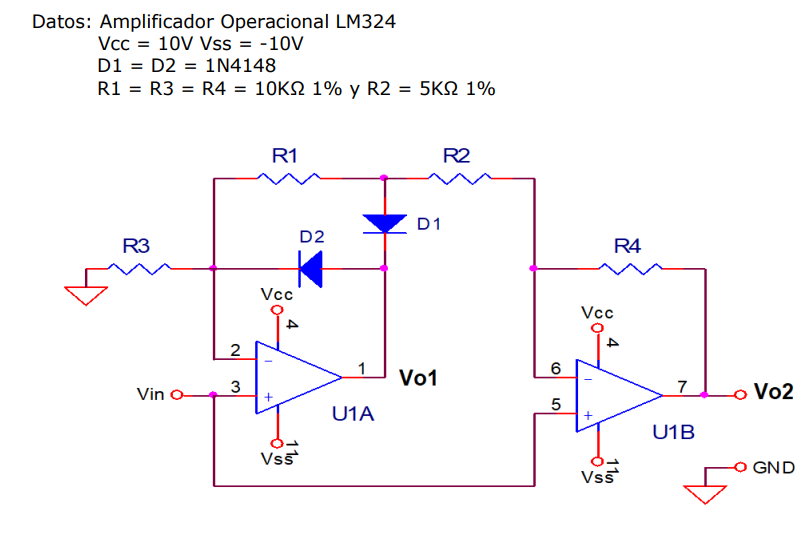
\includegraphics[width=0.5\linewidth]{Secciones/Circuito3/circuito.png}
    \caption{Enter Caption}
    \label{fig:Circuito3}
\end{figure}

\subsection{Análisis Teórico}

Para determinar la tensión de salida Vo en función de la tensión de entrada Vin, se considerarán dos casos: cuando la tensión de entrada es positiva, y cuando la tensión de entrada es negativa.

a) \[V_0 = f(V_{in}) con 0V < V_{in}\]

En estas condiciones, el diodo D2 conduce, mientras que el diodo D1 no, ya que el amplificador U1A se encuentra operando en modo no inversor.
Inicialmente se analizará el caso en que la tensión de entrada del amplificador U1B se encuentra pasivada, entonces la ecuación de corrientes en el nodo ‘6’ resulta:

\begin{equation}
\frac{V_o}{R_4} = \frac{V_in}{R_1 + R_2}
\end{equation}

\begin{equation}
\frac{V_o}{10[k\Omega]} = -\frac{V_{in}}{15[k\Omega]}
\end{equation}

\begin{equation}
V_o = - \frac{2}{3}V_{in}
\end{equation}

Si ahora se pasiva la tensión de entrada del amplificador U1A, se plantea el divisor de tensión en el nodo ‘6’:

\[V_{in} = V_o \frac{R_1+R_2}{R_1+R_2+R_4}\]

\[V_{in} = V_o \frac{15[k\Omega]}{25[k\Omega]}\]

\[V_o = \frac{5}{3}V_{in}\]
Si no se tiene ninguna tensión pasivada, aplicando superposición:

\[V_o = \frac{5}{3}V_{in} - \frac{2}{3}V_{in}\]

\[V_o = V_{in}\]


\subsection{V0 = Vin con 0V > Vin}


En estas nuevas condiciones, el diodo D1 conduce, mientras que el diodo D2 no. Se considerará inicialmente que la tensión a la salida del amplificador U1A se encuentra pasivada. Se plantea el divisor de tensión en el nodo ‘6’:

\[V_{in} = V_o \frac{R_2}{R_2+R_4}\]

\[V_{in} = V_o \frac{5 k\Omega}{15 k\Omega }\]

\[V_o = 3V_{in}\]

Si ahora se considera que la tensión de entrada del amplificador U1B está pasivada, la ecuación de corrientes del nodo ‘6’, tomando VoB como la tensión de salida del amplificador U1B, resulta:

\begin{equation}
\frac{V_{oB}}{R_2} = - \frac{V_o}{R_4}
\end{equation}

\begin{equation}
\frac{V_{oB}}{5 [k\Omega]} = - \frac{V_o}{10 [k\Omega]}
\end{equation}

\begin{equation}
V_o = - 2V_{oB}
\end{equation}

Por otro lado, la tensión de salida VoB se obtiene planteando el divisor de tensión del amplificador U1B:

\[V_{in} = V_{oB} \frac{R_3}{R_1+R_3}\]

\[V_{in} = V_{oB} \frac{10 [k\Omega]}{20 [k\Omega]}\]

\[V_{in} = \frac{1}{2}V_{oB}\]

Reemplazando:

\[V_o = - 4V{in}\]

Si no se tiene ninguna tensión pasivada, aplicando superposición:

\[V_o = 3V{in} - 4V{in}\]

\[V_o = - V{in} \]

En resumen, cuando la tensión de entrada es positiva, la tensión de salida es igual a la tensión de entrada, mientras que cuando la tensión de entrada es negativa, la tensión de salida será positiva y de igual amplitud a la de entrada.


\subsection{Simulacion}
Después de encontrar analíticamente la expresión de la tensión de salida en función de aquella de entrada, simulamos el circuito con el software LTSpice. En el
software, visualizamos la tensión de salida (en verde) para varios valores de tensión de entrada (ver Figuras 25 a 27) y medimos la amplitud de la tensión de salida. Los resultados son reunidos en la tabla de la Figura 28. Para terminar, estos resultados nos permiten graficar la evolución de la amplitud de la señal de salida en función de aquella de la señal de entrada (ver Figura 35 de la sección III.4.).

\begin{figure}
    \centering
    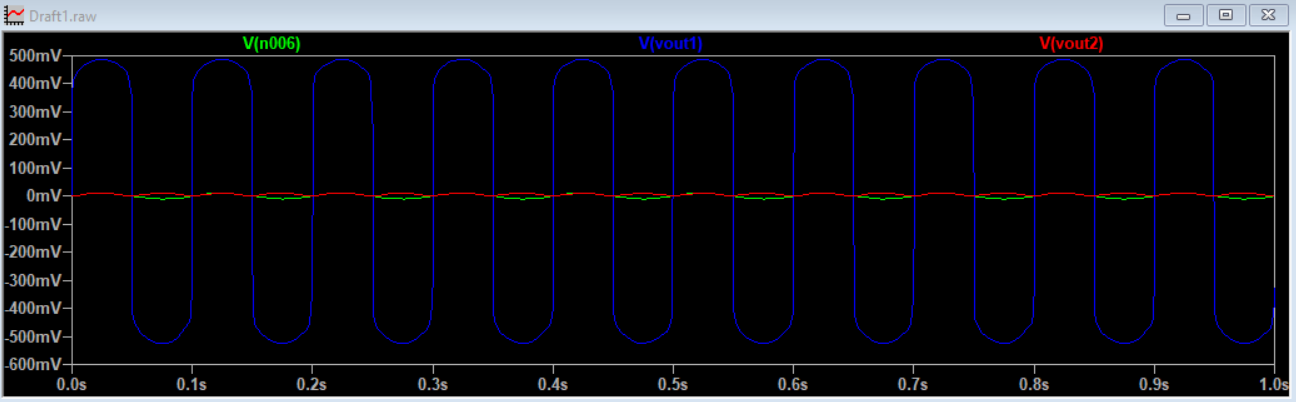
\includegraphics[width=0.5\linewidth]{Secciones/Circuito3/simulacion10mv.png}
    \caption{Enter Caption}
    \label{fig:Simulacion10mv}
\end{figure}

\begin{figure}
    \centering
    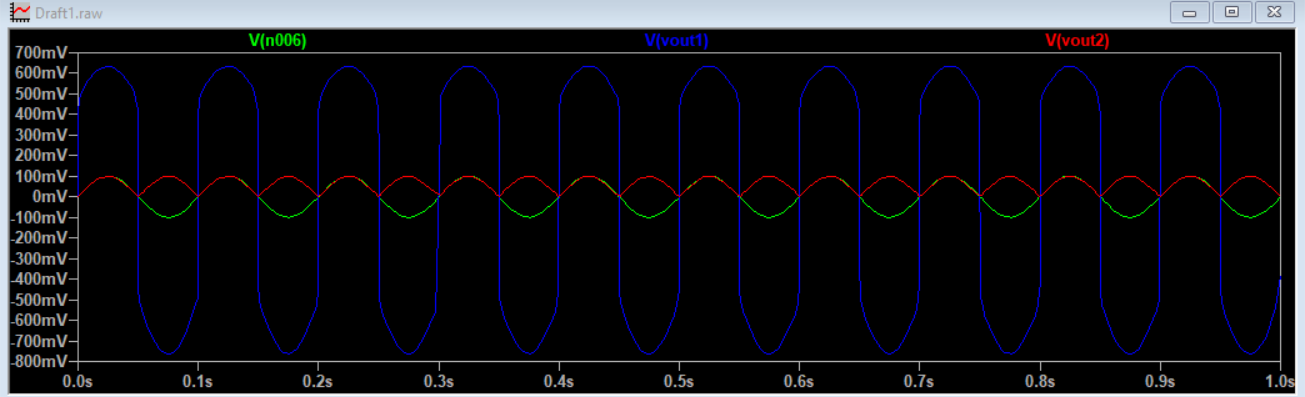
\includegraphics[width=0.5\linewidth]{Secciones/Circuito3/simulacion100mv.png}
    \caption{Enter Caption}
    \label{fig:Simulacion100mv}
\end{figure}

\begin{figure}
    \centering
    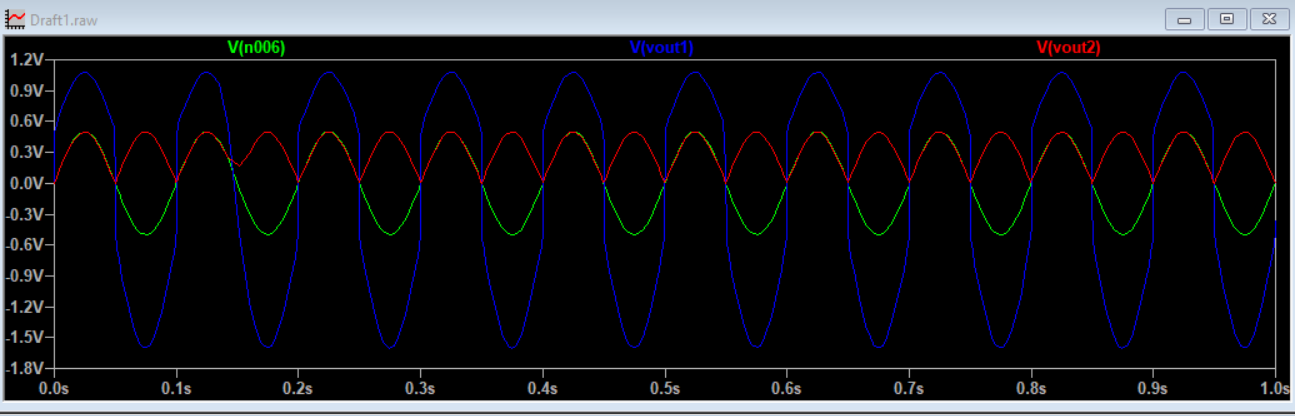
\includegraphics[width=0.5\linewidth]{Secciones/Circuito3/simulacion500mv.png}
    \caption{Enter Caption}
    \label{fig:Simulacion500mv}
\end{figure}

\begin{figure}
    \centering
    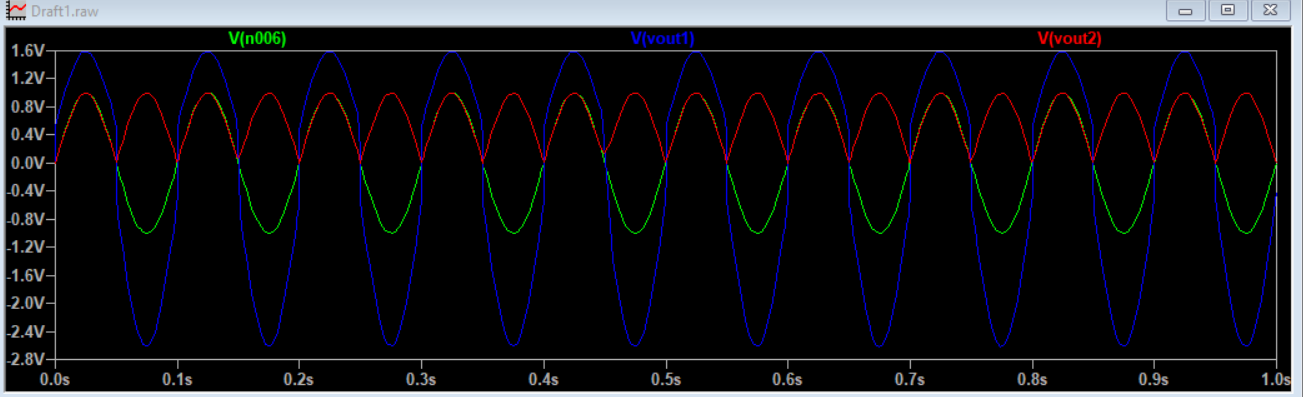
\includegraphics[width=0.5\linewidth]{Secciones/Circuito3/simulacion1v.png}
    \caption{Enter Caption}
    \label{fig:Simulacion1v}
\end{figure}


\begin{figure}
    \centering
    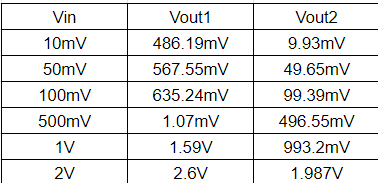
\includegraphics[width=0.5\linewidth]{Secciones/Circuito3/tabla1.png}
    \caption{Enter Caption}
    \label{fig:Tabla1}
\end{figure}

%\subsection{Experimental}

%En el análisis de modo común:




%\subsection{II.4. Comparación de los resultados teóricos, de simulación y experimentales}

%En la siguiente tabla, reunimos los resultados obtenidos por teoricamente, por simulación y experimentalmente. También calculamos los errores relativos entre los resultados obtenidos experimentalmente con los resultados obtenidos por simulación y teóricamente.
%Para Vin=1V y Vin=3V, los errores relativos entre simulación y teoría son extremadamente pequeños (menor a 1%), como previamente. Para esos valores de Vin, los errores exp/simu y exp/teoría quedan bastante pequeños (con un máximo de 10,4%).
%En contrario, podemos ver que para valores más altos de Vin, los errores son mucho más grandes porque ocurre el fenómeno de saturación o sea que la tensión de salida es físicamente limitada por la tensión de alimentación del operador operacional. El gráfico de la Figura 35 permite una mejor visualización de esas conclusiones.


\subsection{Conclusión}
En este trabajo de laboratorio, pudimos estudiar tres circuitos y observar sus limitaciones al momento de armarlos físicamente.
El primero circuito, amplificador de tensión, solamente permite amplificar con una ganancia experimental de un poco más de 3 en vez de 4 como lo esperábamos según el análisis teórico y la simulación.
El segundo circuito, cuando lo armamos físicamente, tuvo un comportamiento parecido a lo que pudimos observar en la simulación y durante el análisis teórico.
Para terminar, el tercer circuito tuvo resultados parecidos a los obtenidos por simulación y análisis teórico para valores de Vin bajos, pero vimos que si
aumentamos demasiado Vin, el circuito está limitado físicamente por el valor de su alimentación y saturación ocurre.